\subsection{Limits for multiplicities}
    Considering difference multisets over an arbitrary abelian group one can notice that some of the surfaces defined by our equations are always the same. There is always the hyperplane $\sum {n_\mu} = k$ and the hypersphere $\sum n_\mu^2 = k + \lambda$ centered at the origin (see Figure \ref{general:figure:surfaces}). 

The second equation confines every multiplicity: $n_\mu \leq \sqrt{k+\lambda}$. By investigating the intersection more thoroughly we discover that the multiplicities are actually bound to be near to their average $k/v$.

    \begin{figure}
        \centering
        \begin{subfigure}[b]{0.5\textwidth}
            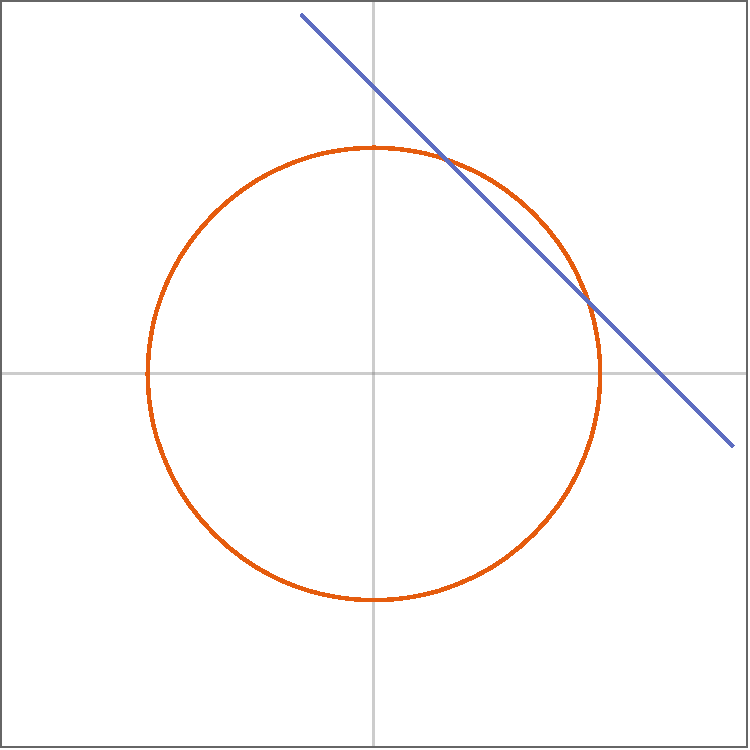
\includegraphics[width=\textwidth]{assets/surfacesIn2D}
        \end{subfigure}%
        ~
        \begin{subfigure}[b]{0.5\textwidth}
            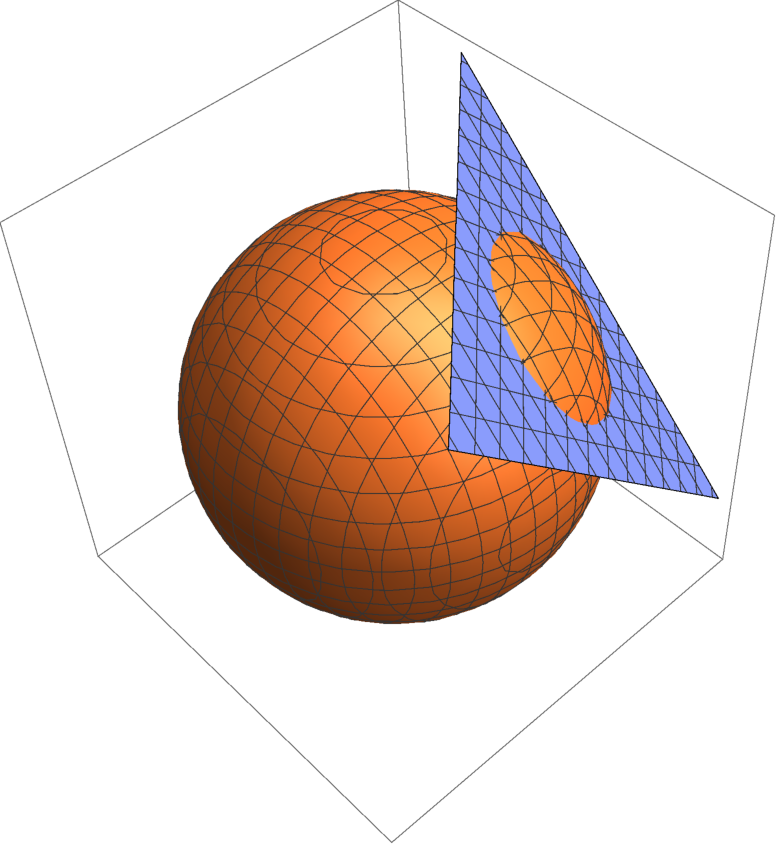
\includegraphics[width=\textwidth]{assets/surfacesIn3D}
        \end{subfigure}
        \caption{The $\sum {n_\mu} = k$ and $\sum n_\mu^2 = k + \lambda$ surfaces in two and three dimensions.}
        \label{general:figure:surfaces}
    \end{figure}
        
    \begin{theorem}
        \label{general:theorem:limits}
        If $M$ is a $(G,k)$-difference multiset and $|G|=v$ then
        \begin{equation}
            \forall \gamma \in G \colon\qquad \frac{k-(v-1)\sqrt k}{v} \leq n(\gamma,M) \leq \frac{k+(v-1)\sqrt k}{v}
        \end{equation}
    \end{theorem}
    
    \begin{proof}
        Take equation \eqref{apparatus:eq:system} for the identity element and equation \eqref{apparatus:eq:ni} as constraints:
        
        \begin{equation}
            \begin{cases}
                \sum {n_\mu} = k \\
                \sum (n_\mu(n_\mu-1)) = \lambda.
            \end{cases}
        \end{equation}
        
        Let us optimize $n_\gamma=n(\gamma,M)$ respecting the constraints. Add the first equation to the second and move all the terms to the left hand side:
        
        \begin{equation}
            \begin{cases}
                k - \sum {n_\mu} = 0 \\
                k + \lambda - \sum n_\mu^2 = 0.
            \end{cases}
        \end{equation}
        
        We apply the method of Lagrange multipliers to obtain the maximum and minimum of $n_\gamma$. 
We use the following Lagrange function ($\lambda_1$ and $\lambda_2$ here is the standard Lagrange multiplier notation and have nothing in common with the parameter $\lambda$).
        
        \begin{equation}
            \mathcal L = n_\gamma - \lambda_1 (k - \sum n_\mu) - \lambda_2 (k + \lambda - \sum n_\mu^2)
        \end{equation}
        
        By a standard application of this method the bounds of the theorem statement are obtained. We omit the routine calculations.
    \end{proof}

    Theorem \ref{general:theorem:limits}
suggests using digressions instead of multiplicities (thus simplifying the equations) and greatly reduces the amount of options for every $n_\gamma$. This simplification allows decent computer searches which enabled us to discover some of the patterns that led to results presented in this paper.
        
    \begin{figure}
        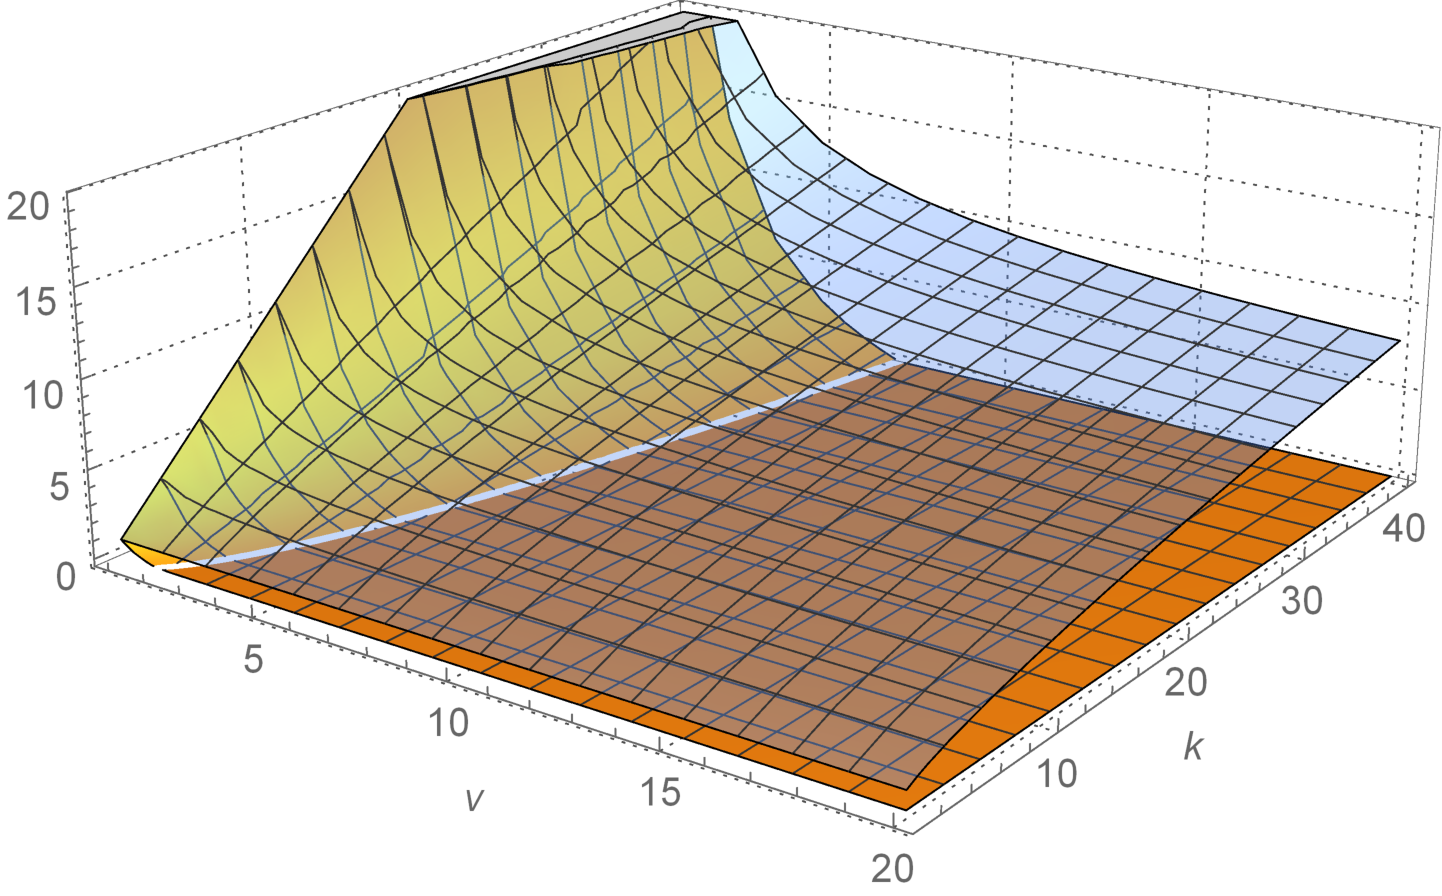
\includegraphics[width=\textwidth]{assets/boundingSurfaces}
        \caption{Lower and upper bounds for the values of $n_\gamma$ with respect to $v$ and $k$.}
        \label{general:figure:limits}
    \end{figure}
    
\subsection{A family of difference multisets for every abelian group}
    
    \begin{theorem}
        \label{regular:theorem:regular}
        If $\sqrt k$ is integer and congruent to $0$ or $\pm 1 \mod v$ then a $(G,k)$-difference multiset exists with the following digressions.
            \begin{itemize}
                \item If $\sqrt k \equiv 1 \mod v$ then $d_\mu = v-1$ for any single element $\mu$ and $d_{\nu \neq \mu} = -1$ for the other elements.
                \item If $\sqrt k \equiv -1 \mod v$ then $d_\mu =1-v$ for any single element $\mu$ and $d_{\nu \neq \mu} = 1$ for the other elements.
                \item Both of the above constructions if $\sqrt k \equiv 0 \mod v$.
            \end{itemize}
    \end{theorem}
    
    \begin{proof}
        The conditions on the values of $k$ and $d_\mu$ guarantee that the multiplicities $n_\mu=\frac{k+d_\mu \sqrt k}v$ are integers. It is left to demonstrate that they form a difference multiset.
        
        Considering equation \eqref{apparatus:eq:dsystem} for non-identity elements we can notice that the digression $\pm(v-1)$ (as any other digression) is involved in two of the products---once as $d_\mu$ and once as $d_{\gamma+\mu}$.

Other $v-2$ products are $(\pm1)\cdot(\pm1)$, thus the condition is satisfied:
        
        \begin{equation}
            \sum d_\mu d_{\gamma+\mu} = 2(\pm(v-1)\cdot(\mp 1)) + (v-2)(\mp1)^2 = -v.
        \end{equation}

        The condition for the identity $\gamma=0$ is also satisfied:
        
        \begin{equation}
            \sum d_\mu^2  = \left( \pm (v-1) \right)^2 + (v-1) \left( \mp 1 \right)^2 = v^2 - v.
        \end{equation}
    
        It is straightforward to check that equation \eqref{apparatus:eq:di} is satisfied as well.
    \end{proof}

\subsection{Difference multisets for cyclic groups}
    Let us consider \eqref{apparatus:eq:dsystem} in matrix form 
    \begin{equation}
    \label{general:eq:matrix_eq}
        D d = \bf v
    \end{equation}\
    where $d = (d_0, d_1, \ldots, d_{v-1})^T$, $\bf{v} = (v^2-v, -v, -v, \ldots)^T$ and $D_{\mu\nu} = d_{\mu+\nu}$, i.e.\ it is the Cayley table of the group in question.
    
    For cyclic groups the matrix $D$ takes the form of an \emph{anticirculant} or \emph{left circulant} matrix:
    
    \begin{equation}
        \label{general:eq:anticirculant_matrix}
        D =
        \begin{pmatrix}
            d_0 & d_1 & d_2 & \cdots & d_{v-1} \\ 
            d_1 & d_2 & d_3 & \cdots & d_0 \\
            d_2 & d_3 & d_4 & \cdots & d_1 \\
            \vdots & \vdots & \vdots & \ddots & \vdots \\
            d_{v-2} & d_{v-1} & d_0 & \cdots & d_{v-3} \\
            d_{v-1} & d_0 & d_1 & \cdots & d_{v-2} \\
        \end{pmatrix}.
    \end{equation}
    
    We will use the discrete Fourier transform:
    \begin{equation}
        \mathcal F (y)_m = \sum_{j=0}^{v-1} y_j \omega^{-jm}
    \end{equation}
    where $\omega = \exp(\frac{2\pi \imath}v)$. Let us consider an equation $Ax=b$ with anticirculant matrix $A$. Applying the discrete Fourier transform to $b$ we obtain
    
    \begin{equation}
        \label{general:eq:fourier_image}
        \mathcal F (b)_m = \mathcal F (a)_m \mathcal F ^*(x^*)_m,
    \end{equation}
    where $a$ is the first row of $A$.
    
    This is particulary useful for equation \eqref{general:eq:matrix_eq} as the vector $d$ is also the first row of matrix $D$. The image of $\bf v=Dd$ is
    
    \begin{equation}
        \mathcal{F} ({\bf v})_m = \mathcal{F}(d)_m \mathcal{F^*}(d^*)_m.
    \end{equation}

    As we are only interested in real $d$, we can simplify it further:
    
    \begin{equation}
        \label{general:eq:dfourier}
        \mathcal{F} ({\bf v})_m = \mathcal{F}(d)_m \mathcal{F^*}(d)_m = |\mathcal{F}(d)_m|^2.
    \end{equation}
    
    Since ${\bf v} = (v^2-v, -v, -v, \ldots)^T$ we can find that $\mathcal{F}({\bf v}) = (0,v^2,v^2,\ldots)$ and \eqref{general:eq:dfourier} becomes
    \begin{equation}
        \label{gen:eq:dfourierfinal}
        \left| \sum_{\mu=0}^{v-1} d_\mu \omega^{-\mu m} \right| = v (1-\delta_{m0})
    \end{equation}

    For any $m | v$ we have $\delta_{m0}=0$ and
    \begin{equation}
        \label{general:eq:split_fourier}
        \left| \sum_{\mu=0}^{v-1} d_\mu \omega^{-m\mu} \right|
        = \left| \sum_{\kappa=0}^{v/m-1} \omega^{-m\kappa} \cdot \sum_{\nu=0}^{m-1}  d_{\kappa+\nu v/m} \right|
        =v
    \end{equation}\
    as 
    \begin{equation}
        \exp\left(\frac{-2\pi \imath m (\kappa+\nu v/m)}v\right) = \exp\left(\frac{-2\pi \imath m \kappa}v\right) \exp\left(-2\pi \imath \nu\right) = \exp\left(\frac{-2\pi \imath m \kappa}v\right)
    \end{equation}
    
    We consider expressions \eqref{gen:eq:dfourierfinal} and \eqref{general:eq:split_fourier} as the main results of this section, here's how one can use it.
    
    \begin{proposition}
        \label{general:theorem:even_cyclic}
        In cyclic groups of even cardinality $\sum_{\mu=0}^{v/2-1} d_{2\mu} = \pm \frac v2$ and $\sum_{\mu=0}^{v/2-1} d_{2\mu+1} = \mp \frac v2$.
    \end{proposition}
    \begin{proof}
        Take \eqref{general:eq:split_fourier} for $m=v/2$
        \begin{equation}
            \left| \sum_{\mu=0}^{v/2-1} d_{2\mu} - \sum_{\mu=0}^{v/2-1} d_{2\mu+1} \right| = v
        \end{equation}
        
        We've split $d$ in half and got that total of one half is by $v$ larger than the total of the other half. The statement of the theorem follows as soon as we remember the grand total $\sum d_\mu = 0$.
    \end{proof}
    
    \begin{remark}
        Similar relation also holds true for some (many? all?) other structures that are not cyclic groups. For example in $\mathbb Z_2 \times \mathbb Z_2$ with elements $\set{\mu, \nu, \zeta, \eta}$ in any order we have $d_\mu+d_\nu-(d_\zeta+d_\eta)=\pm 4$.
    \end{remark}


\subsection{Difference multisets over $\mathbb Z_2^i$}
    \label{sec:z2n}
    We obtained a construction that produces plenty of difference multisets in $\mathbb Z_2^i$. We shall start by explaining the construction and then a proof and analysis of the construction will be presented.

    \subsubsection{Construction}
        Consider the elements $\mu \in \mathbb Z_2^i$ as i-tuples $\mu=(\mu_1, \ldots, \mu_i)$.
        
        Select a hyperplane $H_1$ out of $\mathbb Z_2^i$ defined by equation $0 = a_0 + a_1 \mu_1 + a_2 \mu_2 + \ldots + a_i \mu_i$ ($0=a_0+a\cdot \mu$) with $a_\nu \neq 0$ for at least one $\nu \neq 0$. Set $d_\eta = -1$ for every $\eta \in H_1$.
        
        As for the remaining $(i-1)$-dimensional halfspace: take a hyperplane $H_2$ out of this and set $d_\eta = 3$ for every $\eta \in H_2$.
        
        Repeat this process $0 \leq m \leq i-1$ times setting $d_\eta = \sum\limits_{j=0}^k (-2)^j$ for every $\eta \in H_k$.
        
        You will end up with the final subspace $H_f$ remaining. Select an element $\gamma$ and set $d_\gamma = (-1)^m v + \sum\limits_{j=0}^{m+1} (-2)^j$. Set $d_\eta = \sum\limits_{j=0}^{m+1} (-2)^j$ for the remaining $\eta \in H_f$.
        
        One can also flip the sign on every $d_\mu$ getting another bunch of difference multisets.
        
    \subsubsection{A few examples}
        
        \begin{example}
            Take $i=7$. Thus $v=2^i=128$. Take hyperplane $H_1$ defined by $0=\mu_1$, and set $d_\eta=-1$ for all $\eta\in H_1$ i.e. set $d_{0000000}=d_{0000001}=\ldots=d_{0111111}=-1$.
            
            Let's continue with the remaining subspace ($0=1+\mu_1$). Select another halfpace $H_2$ defined by $0=\mu_2$ and set $d_{1000000}=\ldots=d_{1011111}=3$.
            
            Let's choose $m=4$. We must then repeat the bisections two more times setting $d_\eta=-5$ for $\eta\in H_3$ and $d_\eta=11$ for $\eta \in H_4$.
            
            We have 8 elements left. Let's set $d_{1111111} = (-1)^{m} v + \sum\limits_{j=0}^{m+1} (-2)^j = v - 21 = 107$ and it remains that the other $d_{1111000}=\ldots=d_{1111110}=-21$.
        \end{example}
        
        For tighter examples (with $m\geq i-2$) the multiplicity of the final element will take form of $\sum (-2)^j$ as well. All the digressions will appear to be on the sequence $-1,3,-5,11,-21,43,-85,\ldots$ \cite{A077925}.
        
        \begin{example}
          Take $i=4$ and $m=2$. You will have eight $d_\mu=-1$, four $d_\mu=3$, three $d_\mu=-5$ and one $d_\mu=11$.
        \end{example}
        
        \begin{example}
            \label{2n:example:edge}
            Let's take $i=4$ and $m=3$. You get half the digressions (eight) $d_\mu=-1$. You set another quarter---four digressions $d_\mu=3$. Then you set two $d_\mu=-5$. Halfspace with two elements remains. All except one are set to $d_\mu=11$. And the last one is $-v+11=-5$ Thus you end up with the same set of digressions as in the previous example.
        \end{example}

        Example \ref{2n:example:edge} shows that some of the constructions (the ones with $m=i-1$) produce a difference multiset that coincides with the $m=i-2$ construction.
    
    \subsubsection{Proof}
        For a selected $0 \leq m \leq i-1$ this construction provides us with $2^{i-l}$ digressions of value $d_\eta=\sum\limits_{j=0}^l(-2)^j$ for each $1<l\leq m$ (none of these if $m=0$), $2^{i-m}-1$ digressions equal to $\sum\limits_{j=0}^{m+1}(-2)^j$ and one digression equal to $(-1)^m 2^i+\sum\limits_{j=0}^{m+1}(-2)^j$.
        
        Checking equation $\sum d_\mu = 0$ and $\sum d_\mu^2 = v(v-1)$ is straightforward if you take into account that $\sum\limits_{j=0}^l(-2)^j=(1-(-2)^{l+1})/3$.
        
        Equations \eqref{apparatus:eq:dsystem} are left to check. We began the construction by selecting a hyperplane $H_1$ defined by $0=a_0+a\cdot \mu$ where $a=(a_,a_2,\ldots)$ and $\mu=(\mu_1,\mu_2,\ldots)$ Depending on selection of $\gamma=(\gamma_1,\gamma_2,\ldots)$ there are two cases:
        \begin{itemize}
            \item If $1 \equiv a\cdot \gamma \mod 2$ then $\forall \mu \in H_1 : \mu+\gamma \notin H1 $ and $\forall \mu \notin H_1 : \mu+\gamma \in H1$;
            \item If $0 \equiv a\cdot \gamma \mod 2$ then $\forall \mu \in H_1 : \mu+\gamma \in H1 $ and $\forall \mu \notin H_1 : \mu+\gamma \notin H1$.
        \end{itemize}
        
        In the first case every $d_\mu d_{\mu+\gamma}$ involves factor $-1$. $\sum d_\mu d_{\mu+\gamma} = -2\sum\limits_{i\notin H_1} d_\mu = -2 (\sum d_\mu - \frac v2 (-1)) = -v$.
        
        In the second case $d_\mu d_{\mu+\gamma} = 1$ for every $\mu \in H_1$ and $\sum\limits_{\mu \in H_1} d_\mu d_{\mu+\gamma} = \frac v2$. So the remaining stuff must make up $-\frac {3v}2$ For the remaining stuff we are once again split into two cases depending on $\gamma$ and the initial choice of $H_2$. Either both $\mu$ and $\mu+\gamma$ belong to the different sub-hyperplanes for every $\mu$, or they belong to the same for every $\mu$. That is, we either have $\sum\limits_{j=0}^2 (-2)^j = 3$ in every factor or we continue the process.
        
        In general for any $\gamma$ we will end up at some step where we will have already summed up $d_\mu^2$ for $\mu \in H_1 \cup H_2 \cup \ldots \cup H_r$ and at the next step we will have one of these cases:
        
        \begin{itemize}
            \item No more $H_{r+1}$ has been constructed---only $2^{i-r}-1$ elements with $d_\mu = \sum\limits_{j=0}^{r+1} (-2)^j$ and a single $d_\gamma = (-1)^m 2^i + \sum\limits_{j=0}^{r+1} (-2)^j$;
            \item $\mu \in H_{r+1}$ will have to be multiplied with the items outside $H_{r+1}$ (like the first case in the previous fork).
        \end{itemize}

        The first case checks out:
        \begin{equation}
            \begin{split}
                \sum d_\mu^2 & 
                = \sum\limits_{H_1 \cup \ldots \cup H_r} d_\mu^2 \\
                & + (2^{i-r}-2) \left(\sum\limits_{j=0}^{r+1} (-2)^j \right)^2 \\
                & + 2 \left(\sum\limits_{j=0}^{r+1} (-2)^j \right) \left( (-1)^r 2^i + \sum\limits_{j=0}^{r+1} (-2)^j \right) \\
                = & - 2^i = -v
            \end{split}
        \end{equation}
    
        The second does as well:
        \begin{equation}
            \begin{split}
                \sum d_\mu^2 & \\
                = & \sum\limits_{H_1 \cup \ldots \cup H_r} d_\mu^2 \\
                + & 2 \left(\sum\limits_{j=0}^{r+1} (-2)^j \right) 
                 \Bigg(
                    \sum\limits_{l=r+2}^{m} 2^{i-l} \sum\limits_{j=0}^l (-2)^j \\
                   & + (2^{i-m}-1)\sum\limits_{j=0}^{m+1} (-2)^j \\
                   & + (-1)^m 2^i + \sum\limits_{j=0}^{m+1} (-2)^j
                 \Bigg) \\
                = & - 2^i = -v
            \end{split}
        \end{equation}
    
    \subsubsection{Analysis}
        For $i \leq 3$ the construction makes all the difference multisets there are. This can be shown explicitly by solving the digression equations.
        
        We don't know about larger groups. Our construction produces $2^i$ different values for $i \leq 3$ but only 12, 16 and 20 different $d_\mu$ values for $i$ of 4,5 and 6 respectively.
        
        As for the number of difference multisets, this construction produces
        \begin{equation}
            2 \sum\limits_{j=2}^i 2^j \prod\limits_{l=j+1}^i (2^{l+1}-2)
        \end{equation}\
        solutions for $d_\mu$ over $\mathbb Z_2^i$. The counting argument is that we can select $H_1$ in $2^{i+1}-2$ ways, $H_2$ in $2^i-2$ etc. until you stop and choose one of the remaining $2^j$ elements. And twice everything as you can flip the signs.
        
        The difference multisets (i.e.\ integer solutions $n_\mu=\frac{k+d_\mu \sqrt k}v$) themselves are produced whenever $v | \sqrt k$. In addition the cases of single $d_\gamma = \pm (v-1)$ and the rest $d_\mu = \mp 1$ we get integer $n_\mu$ for $k \equiv \mp 1 \mod v$.
        
\subsection{Difference multisets over the three element group}
    \label{sec:z3}
    There is only one group of three elements. Let's take it in form of $\mathbb Z_3$. What must the $k$ be for $(\mathbb Z_3,k)$-difference multiset to exist? What are these difference multisets and how many of them are there for a particular value of $k$?

    To answer these questions we shall write down \eqref{apparatus:eq:system} for a non-identity element and combine it with \eqref{apparatus:eq:ni} and \eqref{apparatus:eq:parameters} to form a system of equations.

    \begin{equation}
        \label{v3:eq:constraints}
        \begin{cases}
            3\lambda = k(k-1) \\
            \sum n_\mu = k \\
            \sum n_\mu n_{\mu+1} = \lambda
        \end{cases}
    \end{equation}

    We may now combine the equations to discover a relation between multiplicities of elements.

    \begin{theorem}
        \label{v3:theorem:relations}
        Multiplicities of different $(\mathbb Z_3,k)$-difference multiset elements $\mu$ un $\nu$ are related via
        \begin{equation}
            \label{v3:eq:relations}
            n_{\mu\neq \nu} = \frac{k-n_\nu \pm \sqrt{\frac{4k-(k-3n_\nu)^2}{3}}}{2}
        \end{equation}
    \end{theorem}

    \begin{proof}
        Take any element $\gamma \in \mathbb Z_3$ and assign $c = n_\gamma$. Let's use $\alpha$ and $\beta$ to name the remaining elements of $\mathbb Z_3$. The system \eqref{v3:eq:constraints} can now be rewritten:
        \begin{equation}
            \begin{cases}
                n_\alpha + n_\beta = k - c \\
                n_\alpha n_\beta + c (n_\alpha + n_\beta)  = \lambda 
            \end{cases}
        \end{equation}
        
        Substitute $k'=k-c$ and $\lambda' = \lambda + c^2-kc$ to obtain
        
        \begin{equation}
            \begin{cases}
                n_\alpha + n_\beta = k' \\
                n_\alpha n_\beta = \lambda'
            \end{cases}
        \end{equation}
        
        Eliminating $n_\beta$ we arrive at a quadratic equation that is solved into
        
        \begin{equation}
            n_\alpha = \frac{k' \pm \sqrt{k'^2-4\lambda'}}{2}
        \end{equation}
        
        Undo the substitutions and you're done.
    \end{proof}

    Considering the multiplicities in form of $n_\mu = \frac{k+\Delta_\mu}{3}$, we can restate \eqref{v3:eq:relations} into the following.

    \begin{equation}
        \label{v3:eq:relations_delta}
        n_{\mu\neq \nu} = \frac{k-n_\nu \pm \sqrt{\frac{4k-\Delta_\nu^2}{3}}}{2}
    \end{equation}

    The rest of analysis focuses on the $\Delta_\mu$ and it's effect on the above equation. The behaviour of expression under the root is tied to a topic in number theory called Löschian numbers \cite{oeisA003136}. These numbers make an appearance in a variety of fields (see comments in \cite{oeisA003136}).

    \begin{definition}
        \label{v3:def:loeshian}
        Number $k$ is called a Löschian number if $\exists a,b \in \mathbb Z \colon a^2+ab+b^2=k$.
    \end{definition}

    For our purposes (to eliminate unnecessary symmetries) we will only consider $a,b$ such that $a \geq b \geq 0$. This, however, doesn't change the scope of Löschian numbers.

    \begin{lemma}
        \label{v3:lemma:loeschian}
        For any Löschian number $k$ we can find $a,b \in \mathbb Z$ such that $a^2+ab+b^2=k$ and $a \geq b \geq 0$.
    \end{lemma}

    \begin{proof}
        As $k$ is a Löschian number there are $a',b' \colon a'^2+a'b'+b'^2=k$. We can construct $a,b$ such that $a^2+ab+b^2=k$ and $a \geq b \geq 0$ as follows:
        \begin{itemize}
            \item If $a' \geq 0$ and $b' \geq 0$ just take $a=a'$ and $b=b'$ or swap them if $a'<b'$.
            \item If $a'<0,b'<0$ take $a'=-a,b'=-b$ or swap them if $a'>b'$.
            \item If $ab<0$ take either $a'=|a|, b'=|a+b|$ or $a'=|a+b|, b'=|b|$. Swap places as necessary to ensure $a \geq b \geq 0$.
        \end{itemize}
    \end{proof}

    Having introduced the term, we may now introduce the promised link.

    \begin{lemma}
        \label{v3:lemma:square}
        There exists a $\Delta$ that makes $\frac{4k-\Delta^2}{3}$ a perfect square iff $k$ is Löschian number.
        
        $\Delta$ values that does the job are $\pm (2a+b), \pm (a+2b), \pm (a-b)$, where $a,b$ are such that $a \geq b \geq 0$ and $a^2+ab+b^2=k$. There is no other $\Delta$ that makes $\frac{4k-\Delta^2}{3}$ into square.
    \end{lemma}

    \begin{proof}
        For a Löschian number $k=a^2+ab+b^2$ take $\Delta$ equal to $\pm (2a+b)$, $\pm (a+2b)$ or $\pm (a-b)$ and obtain the value of expression in question to be $b^2$, $a^2$ or $(a+b)^2$ which are clearly squares.
        
        On the other hand, if $\frac{4k-\Delta^2}{3}$ is square, assign:
        \begin{equation}
            z^2 = \frac{4k-\Delta^2}{3}
        \end{equation}
        
        Rewrite
        \begin{equation}
            \frac{3z^2 + \Delta^2}{4} = k
        \end{equation}
        
        Noticing that $4$ divides $3z^2 + \Delta^2$ we can conclude that $z$ and $\Delta$ are of the same parity (because $z^2 \equiv \Delta^2 \mod 4$). Thus $2$ divides both $\Delta-z$ and $\Delta+z$.
        
        We can now find integers $a,b$ such that $a \geq b \geq 0$ and $a^2+ab+b^2=k$ (thus $k$ is a Löschian number) and the $\Delta$ can be expressed in one of the expressions stated in lemma.
        
        \begin{itemize}
            \item If $z \geq \Delta$ take $a=\frac{z+\Delta}{2}$ and $b=\frac{z-\Delta}{2}$. Then $a-b=\Delta$.
            \item If $\Delta \geq z \geq \frac \Delta 3$ take $a=z$ and $b=\frac{\Delta-z}{2}$. Then $a+2b=\Delta$.
            \item If $\frac \Delta 3 \geq z$ take $a=\frac{\Delta-z}{2}$ and $b=z$. Then $2a+b=\Delta$.
        \end{itemize}
    \end{proof}

    Let's introduce the following notation for the three values used in lemma \ref{v3:lemma:square}. The rest can be expressed as $-\Delta_i$:
    \begin{equation}
        \label{v3:eq:deltas}
        \Delta_\alpha = 2a+b, \Delta_\beta = -a-2b, \Delta_\gamma = -a+b
    \end{equation}

    These $\Delta_i$ will be used in the following theorem and $\alpha$, $\beta$ and $\gamma$ are labels that, as before, we use to label the elements of $\mathbb Z_3$ in arbitrary order. We can now state our main result which is both construction and existence criterion for $(\mathbb Z_3,k)$-difference multisets.

    \begin{theorem}
        \label{v3:theorem:loeschian}
        For every pair $a,b \in \mathbb Z$ such that $k=a^2+ab+b^2$ and $a \geq b \geq 0$ there are exactly $-(k+1) \mod 3$ (up to automorphisms) $(\mathbb Z_3,k)$-difference multisets and the multiplicities of their elements are
        
        \begin{itemize}
            \item $n_\mu=\frac{k+\Delta_\mu}{3}$ for one and $n_\nu=\frac{k-\Delta_\nu}{3}$ for the other if $3 \mid k$.
            \item $n_\mu=\frac{k+\Delta_\mu}{3}$ if $3 \nmid k$ un $b-a \equiv 1 \mod 3$.
            \item $n_\mu=\frac{k-\Delta_\mu}{3}$ if $3 \nmid k$ un $a-b \equiv 1 \mod 3$.
        \end{itemize}
    \end{theorem}

    \begin{proof}
        According to lemma \ref{v3:lemma:square}, the expression \eqref{v3:eq:relations_delta} will equal integer only if $k$ is a Löschian number and $\Delta_\mu$ is one of the listed on \eqref{v3:eq:deltas} or a negative of that.
        
        Insert the constructions listed in \eqref{v3:theorem:loeschian} into \eqref{v3:eq:relations} to check that these are indeed multiplicities that make up a difference multiset if the numbers are whole. One can also check that using $\Delta_\alpha$ to construct one of the multiplicities you will find $\Delta_\beta$ and $\Delta_\gamma$ used for the others and the same is true in any order.
        
        Considering remainders one may check the following:
        \begin{itemize}
            \item If $a \equiv b \mod 3$ then $3 \mid k$ and all the multiplicities in both the constructions $n_\mu=\frac{k+\Delta_\mu}{3}$ and $n_\mu=\frac{k-\Delta_\mu}{3}$ are integers.
            \item If $a \equiv b-1 \mod 3$ then $k \equiv 1 \mod 3$ and only the multiplicities constructed by $n_\mu=\frac{k+\Delta_\mu}{3}$ are all integer.
            \item If $a \equiv b+1 \mod 3$ then $k \equiv 1 \mod 3$ and only the multiplicities constructed by $n_\mu=\frac{k-\Delta_\mu}{3}$ are all integer.
        \end{itemize}
    \end{proof}

    \begin{remark}
        Allowing $a,b$ such that $a \geq b \geq 0$ wouldn't hold, we'd obtain the same $\Delta_\alpha, \Delta_\beta, \Delta_\gamma$ in different order thus making the same difference multisets again (up to automorphism). This constraint is intended to exclude such symmetries.
        Different $a \geq b \geq 0$ pairs with $a^2+ab+b^2=k$ will lead to different value of $a-b$ and thus all the constructions mentioned in \ref{v3:theorem:loeschian} will be distinct. Consequently the number of $(\mathbb Z_3,k)$ will be proportional to number of unique $a,b$ pairs (respecting constraints) and the coefficient of proportionality is $-(k+1) \mod 3$.
    \end{remark}

    \subsection{Estimating numbers}
        Despite our effort, the exact number of solutions is still elusive. This aspect is now reduced to a number-theoretic question -- how many unique solutions are there for $k=a^2+ab+b^2$ such that $a\geq b\geq 0$.

        The number of solutions without the constraint is known \cite{marmon2005hexagonal}. Denote
        \begin{equation}
            k=3^\alpha p_1^{\alpha_1}p_2^{\alpha_2}\ldots q_1^{\beta_1}q_2^{\beta_2}\ldots
        \end{equation}\
        
        where $p_i$ are primes such that $p_i \equiv 1 \mod 3$ and $q_i$ are primes such that $q_i \equiv 2 \mod 3$. If any of the $\beta_i$ are odd, there are no integer solutions to $k=a^2+ab+b^2$. But if all of $\beta_i$ are even, the number of solutions is $6\prod (\alpha_i +1)$.
        
        It is hypothesised \cite{nair2004elementary} that the number of solutions (if every $\beta_i$ is even) having $a \geq b \geq 0$ is $1/2 + \prod (\alpha_i +1)/2$ if all the $\alpha_i$ are even and $\prod (\alpha_i +1)/2$ otherwise. We checked this to be true for a thousand Löschian numbers. However, for most of the Löschian numbers this remains unchecked.
